% CONFIGURATIONS
\documentclass{article}
\usepackage{array}
\usepackage{parskip} % For paragraph layout
\usepackage{setspace} % For using single or double spacing
\usepackage{emptypage} % To insert empty pages
\renewcommand{\arraystretch}{1.5} % Spazio extra per centratura verticale
\newcolumntype{C}[1]{>{\centering\arraybackslash}m{#1}}
\usepackage{multicol} % To write in multiple columns (executive summary)
\setlength\columnsep{15pt} % Column separation in executive summary
\setlength\parindent{0pt} % Indentation
\raggedbottom  

% PACKAGES FOR IMAGES
\usepackage{graphicx}
\usepackage{transparent} % Enables transparent images
\usepackage{eso-pic} % For the background picture on the title page
\usepackage{subfig} % Numbered and caption subfigures using \subfloat.
\usepackage{tikz} % A package for high-quality hand-made figures.
\usetikzlibrary{}
\graphicspath{{./Images/}} % Directory of the images
\usepackage{caption} % Coloured captions
\usepackage{amsthm,thmtools,xcolor} % Coloured "Theorem"
\usepackage{float}

% PACKAGES FOR TABLES
\usepackage{tabularx}
\usepackage{xltabular}
\usepackage{booktabs}
\usepackage{longtable} % Tables that can span several pages
\usepackage{colortbl}

% OTHER PACKAGES
\usepackage{pdfpages} % To include a pdf file
\usepackage{afterpage}
\usepackage{lipsum} % DUMMY PACKAGE
\usepackage{fancyhdr} % For the headers
\fancyhf{}

\begin{document}

% Title Page
\title{RASD Document}
\author{Alessandro Salvatore, Erdal Yalçın, Leonardo Ratti}
\date{Academic Year: 2024-25}
\maketitle

% Table of Contents
\newpage
\tableofcontents

% Sections (These are examples, replace with actual content as needed)
\newpage
\section{Introduction}
\subsection{Purpose}
Students\&Companies (S\&C) is a dynamic platform designed to connect university students seeking internships with companies offering valuable opportunities. By leveraging students' skills, experiences, and career interests alongside the specific needs and offerings of companies, S\&C aims to create seamless matches. The platform provides a recommendation system that notifies students about relevant internships and informs companies of suitable candidates. It also facilitates the selection process, supports feedback exchange, and helps both parties refine their profiles for better alignment. S\&C results useful thanks to the offered tools for monitoring internship progress and resolving issues collaboratively.
\subsubsection{Goals}
The goals specify what the platform will allow users to achieve in the real world, everything else will not be allowed. 
\\All the starred words will be defined in section 1.3 to avoid any ambiguity.
\begin{itemize}
  \item \textbf{G1} Allows registered companies* to post* and advertise* the available internships that they offer.
  \item \textbf{G2} Allows registered students* to proactively and autonomously search and apply* to advertised internships.
  \item \textbf{G3} Helps registered students and registered companies by suggesting them appealing templates for their CVs and internship projects drafts.
  \item \textbf{G4} Allows a registered student to be recommended a list of advertised internships that might be of interest to him/her with respect to: his/her uploaded CV, the internships projects* and users'* feedbacks.
  \item \textbf{G5} Allows a registered company to be recommended a list of registered students who might be of interest for one of its advertised internships with respect to: their uploaded CVs, the internship project and users' feedbacks.
  \item \textbf{G6} Allows a registered company to view the list of all the students who applied to one of its advertised internships grouped by the internship they applied to.
  \item \textbf{G7} Allows a company to get in contact* with the candidates* for one of its internships and, only after, manage their selection process*.
  \item \textbf{G8} Allows registered companies and students that are taking part* in an ongoing internship to comment about it.
  \item \textbf{G9} Allows a registered university to view the comments about an ongoing internship, written either by its interning students or by the host company.
  \item \textbf{G10} Allows a registered university to interrupt an ongoing internship involving one its students.
      \item \textbf{G11} Allows companies and students to provide feedback about a past internships only if they respectively offered it and took part in it.

\end{itemize}
\subsection{Scope}
\subsubsection{World Phenomena}
    \begin{itemize}
        \item \textbf{W1} A company wants to advertise an internship. 
        \item \textbf{W2} A student wants to find an internship opportunity.
        \item \textbf{W3} A student wants to discover interesting companies.
        \item \textbf{W4} A company wants to interview the internship candidate and select them.
        \item \textbf{W5} A student wants to evaluate an internship process
        \item \textbf{W6} A company and a student want to improve the internship advertisement and the CV, respectively.
        \item \textbf{W7} A University wants to follow an internship process
    \end{itemize}
\subsubsection{Shared Phenomena}
    \textit{Controlled by World}
    \begin{itemize}
        \item \textbf{S1} A student searches for internships on the platform.
        \item \textbf{S2} A company posts an internship advertisement on the platform.
        \item \textbf{S3} A student selects and accepts internships he wants to make contact with.
        \item \textbf{S4} A company selects and accepts a number between all the interested and recommended students as candidates for the given internship.
        \item \textbf{S5} A Student or a Company sends information of any type about the state of an on-going internship, like complaining or providing general information.
        \item \textbf{S6} A University interrupts an internship of a student after some complaints from the company or from the student. 
        \item \textbf{S7} A user registers either as Student, Company or University.
        
        \item \textbf{S1} A registered student submit their resumes on the S\&C.
        \item \textbf{S2} A registered company advertises an internship opportunity on S\&C.
        \item \textbf{S3} A company selects a student through the S\&C based on interesting skills from the student's CV. 
        \item \textbf{S4} A student selects the internship they want to apply for through the S\&C.
        \item \textbf{S5} A company creates interview request through the S\&C for the interview, after the match.
        \item \textbf{S6} A student and a company are able to provide feedback on their experiences, after the selection process.
        \item \textbf{S7} A company offers an internship position to the relevant student through the S\&C.
        \item \textbf{S8} A student accepts or declines an internship position through the S\&C.
        \item \textbf{S9} A student's university follows up on feedback about the internship process through the S\&C and is able to interrupt the internship if necessary.
        \item \textbf{S10} A student updates their resume based on the suggestions received from the S\&C.
        \item \textbf{S11} A student updates their advertisement based on the suggestions received from the S\&C.
    \end{itemize}
    \textit{Controlled by Machine}
    \begin{itemize}
        \item \textbf{S12} The system notifies a company about an interesting student resume.
        \item \textbf{S13} The system notifies to a student an internship that might interest him is available.
        \item \textbf{S14} The system starts a contact process when both an internship and a student confirm an interest in each other.
        \item \textbf{S15} The system shows some information about a student profiles to a company.
        \item \textbf{S16} The system shows some information about an internship advertisement and a company profile to a student.
        \item \textbf{S17} The system notifies a student when the interview date is scheduled.
        \item \textbf{S18} The system creates an interview link and sends to the both sides.
        \item \textbf{S19} The system analyzes the feedback data and provides suggestions for improving the profiles. 
        \item \textbf{S20} The system recommends interesting profiles and shows to the both sides.
        \item \textbf{S21} The system notifies a student when the company's decision is announced.
        \item \textbf{S22} The system creates a link for following and handling the internship process and sends to the student's university.
        \item \textbf{S23} The system notifies a student when internship is advertised from a favorite company which has manually searched for.
    \end{itemize}
\subsection{Definitions, Acronyms, Abbreviations}

\subsubsection{Definitions}
    \begin{itemize}
        \item Recommendation: It's a platform feature that starts a matching between a company and a student. If both parties accept the recommendation, the student is taken for the selection process
        \item Accepting: The act of students or companies, who got recommended to each other, to confirm their interest. 
        \item Selection: It's the process that starts after the expiration date of applying for the internship. The company interviews every accepted student and picks the best one(s) for their needs. 
        \item Feedback: Refers to the comments and questionary that both parties are asked to fill in at the end of the internship contract, in order to improve the platform.
        \item Observation: Is anything written in the dedicated Observations section. Serves the student or the company currently engaged, to highlight something about the experience with each other. If that's a complaint from either, the University of the student will manage the situation.
        \item Complaint: It's a specific type of Observation, where the University of the student is called to act and manage the situation between the parties.
        \item Contact: The mutual acceptance between student and company.
    \end{itemize}
\subsubsection{Acronyms}
    \begin{itemize}
        \item S\&C: "Students\&Companies", the name of the platform
    \end{itemize}
\subsubsection{Abbreviations}
    \begin{itemize}
        \item Wn: n-th World Phenomena
        \item Sn: n-th Shared Phenomena
        \item Gn: n-th Goal
        \item Dn: n-th Domain Assumption
        \item Rn: n-th Requirement
    \end{itemize}
\subsection{Revision history}
\subsection{Reference Documents}
    \begin{itemize}
        \item Software Engineering 2 A.Y. 2024/2025 Slides (course material)
        \item Assignment RDD A.Y. 2024/2025 (Requirement Engineering and Design Project: goal, schedule, and rules)
    \end{itemize}

\subsection{Document Structure}
    This document is composed of six sections:

\begin{itemize}
    \item \textbf{1st Chapter}: We begin by presenting the problem statement and outlining the system's objectives. In the scope subsection, we offer insights into the various real-world and shared phenomena that the system addresses. Finally, we provide essential resources for readers, including definitions and abbreviations, to facilitate a comprehensive understanding of this document.
    
    \item \textbf{2nd Chapter}: We offer a comprehensive overview of the system, including insights into User profiles and their primary functions. We also establish the key domain assumptions underpinning the system's operation.
    
    \item \textbf{3rd Chapter}: We delineate the system's requirements, encompassing both functional and non-functional aspects. In addition, we present Use Case Diagrams that illustrate system interactions, accompanied by detailed descriptions of each use case and related Sequence Diagrams. Lastly, we establish a clear mapping of these requirements to both system goals and use cases for comprehensive understanding.
    
    \item \textbf{4th Chapter}: We provide a formal analysis of the system to be with Alloy.
    
    \item \textbf{5th Chapter}: We provide an estimate of the effort spent by each group member.
    
    \item \textbf{6th Chapter}: We provide a list of the references used in this document.
\end{itemize}

\section{Overall Description}
\subsection{Product Perspective}
\subsubsection{Scenarios}
    \begin{itemize}
        \item 1st Scenario: Signing up. User John has accessed the opening page; he registers into the site as a student, filling the required data and is sent back to the opening page.
        \item 2nd Scenario: Logging in. User John is in the opening page; he logs into the site using his credentials, and can now access to his possible operations.
        \item 3rd Scenario: Finalizing registration. The student John opens his profile page and uploads his CV document into the platform; he studies at Polime, so he connects his university mail with his account.
        \item 4th Scenario: Starting an offer. The company Emazon posts an internship offer on the platform, deciding the expiration date and the duration of it. Then Emazon lists the tasks the student will have to perform, the application domain and other relevant things regarding the internship.  
        \item 5th Scenario: Platform recommendation. Upon CV uploading, the   platform analyzes John's CV and automatically suggests him all the current potential interesting internship offers. After Emazon has posted its internship offer, it gets notified to him too.
        \item 6th Scenario: Searching Internships. John opens the page of the available internships. He filters out the ones without benefits, and is left with few options. He applies for Guggl's offer.
        \item 7th Scenario: Student accepts recommendation. John gets the
        notification from Emazon and decides to accept it.
        \item 8th Scenario: Company accepts students. After Emazon posted the internship offer, it gets recommended some students by the platform, while some other students found the internship by manual searching. Emazon accepts John and some other students.
        \item 9th Scenario: Entering the selection. After the expiration date passes, the company starts the selection process. Emazon proposes the interviews dates and time schedules through the dedicated interface to all the contacted students.
        \item 10th Scenario: Student chooses interview day. Since John has established contact with Emazon, he selects the time and day of the interview through the dedicated interface.
        \item 11th Scenario: Student joins the interview. When the scheduled day for the interview comes, John can meet the interviewer using the link posted by the company on the platform. After some time, the platform officially notifies him that he was selected.
        \item 12th Scenario: Writing Observations. Emazon writes a complaint in the provided space about John's current behaviour.
        \item 13th Scenario: University acts. The University Polime gets a complaint from Emazon about John's behaviour. Polime decides to interrupt his internship.
        \item 14th Scenario: Giving Feedback. At the end of the internship, John and Emazon fill a questionnaire about their experience with the platform and give suggestions to it.
    \end{itemize}
\subsubsection{Class Diagram}
The UML Class Diagram shown below provides a conceptual, high-level representation of the intended software. At this stage, it may include entities that will not necessarily be part of the final system. Additionally, this diagram intentionally omits methods and other detailed elements that will be addressed in the design phase.
\\The three main components are User, Internship and Student\&Company (which represents the software itself). They are connected with arrows in order to recreate the interactions between one another. The User views the Internship according to his granted permissions. Then he/she interacts with the platform (i.e. accepts a recommendation, submits feedback... ) and eventually the system accordingly manages the Internship.
\begin{figure}[H]
    \centering
    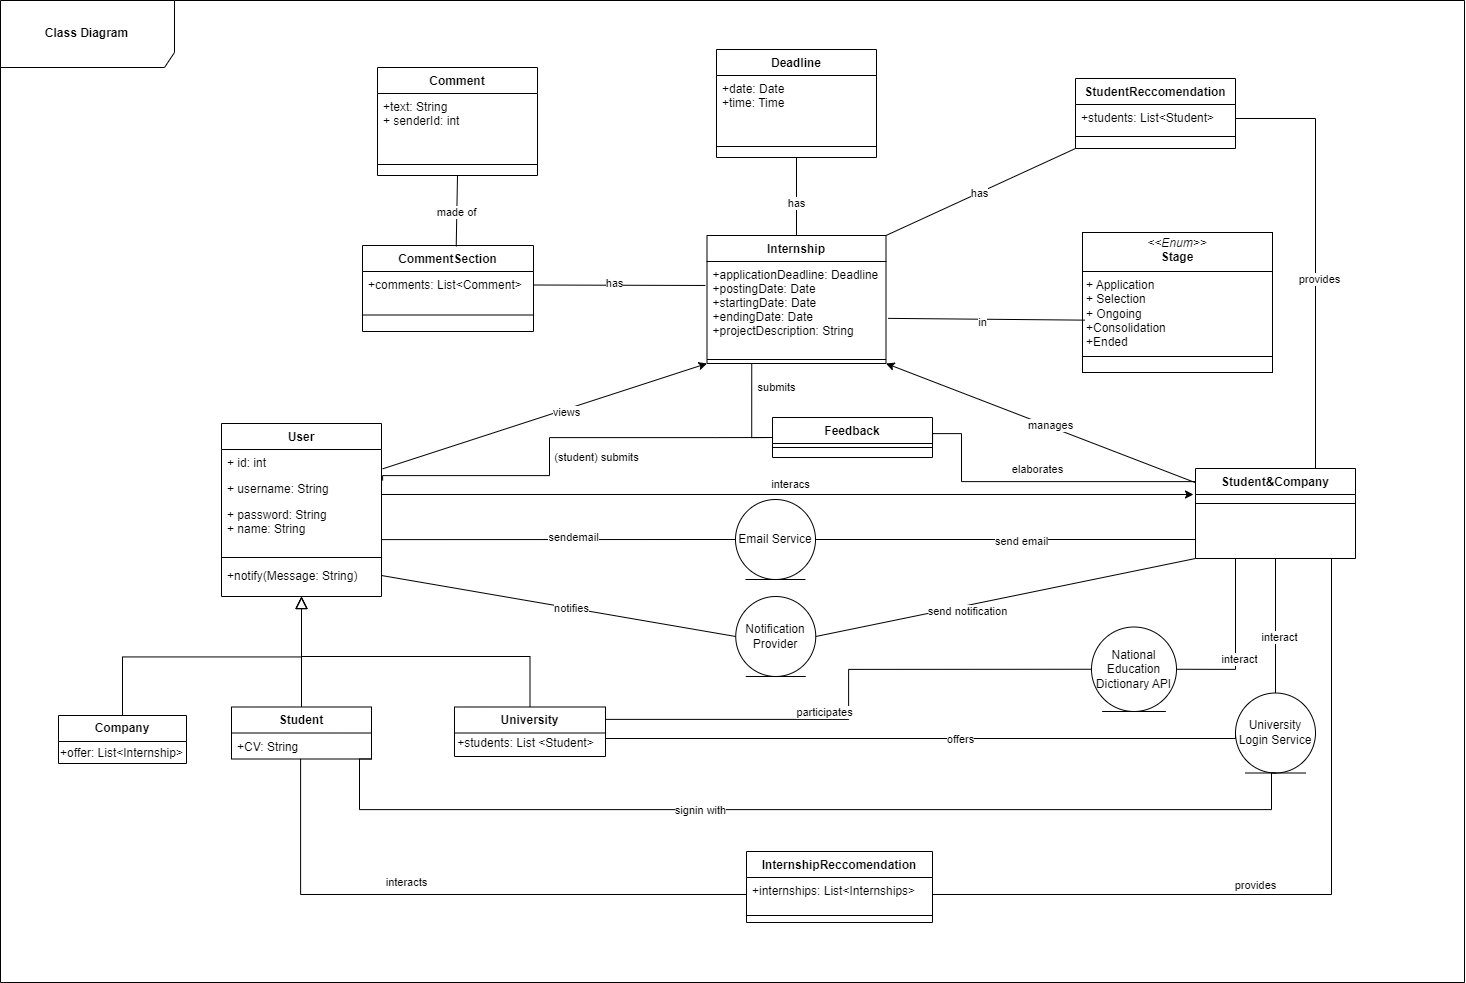
\includegraphics[scale = 0.30]{figures/Class Diagram.drawio.png}
    \centering
\end{figure}
\subsubsection{State Charts}
The following section outlines the key component (Internship) of the Student\&Company (S\&C) system and its evolution across different phases. To illustrate this, the UML State Chart is presented.
\begin{figure}[H]
    \centering
    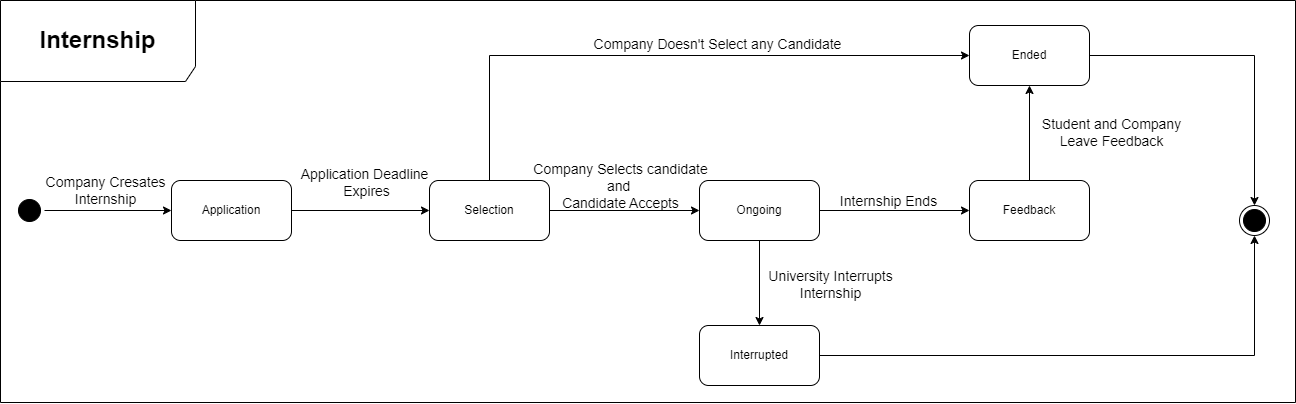
\includegraphics[scale = 0.30]{figures/StateCharts.drawio.png}
    \centering
\end{figure}
The diagram in question outlines the potential phases of an Internship. Posted by a Company, the Internship promptly enters the "Application" state, allowing Students to apply and Companies/Students to accept recommendations. 
\\Following the closure of the application window, the system transitions the Internship to the "Selection" state, in which the Candidates are interviewed, selected and confirmed. 
\\In case no Candidate is confirmed, the Internship is archived and transitioned to the "Ended" state. Otherwise, the selected Candidate starts the interning period and the Internship is changed into the "Ongoing" state. 
\\While the Internship is "Ongoing" and the University responsible for the Student receives complaints, it may decide to terminate the Internship. In such cases, the Internship is moved to the "Interrupted" state and archived as is.
\\If the Internship ends without interruptions, before being archived, it waits for both the selected Candidate and the host Company to provide a feedback about the interning experience. The Internship is therefore placed in its "Feedback" state.
\\Only afterwards, the system closes the Internship, transitioning it in the "Ended" state and archiving it.


\subsection{Product Functions}
\subsubsection{Requirements}
    \begin{itemize}
        \item \textbf{Requirement} Students can share their CVs on the platform
        \item \textbf{R1} The system must allow a student who wants to register to sign up.
        \item \textbf{R2} The system must allow a company who wants to register to sign up.
        \item \textbf{R3} The system must allow a university who wants to register to sign up.
        \item \textbf{R4} The system must allow registered users to sign in using their credentials.
        \item \textbf{R5} The system must allow registered users who wishes to reset their password to change it after completing various procedures and checks.
        \item \textbf{R6} The system must be able to send notifications to all users.
        \item \textbf{R7} The system must allow registered students to enter information from their CV to complete their profiles.
        \item \textbf{R8} The system must allow registered companies to post internship advertisements.
        \item \textbf{R9} The system must allow companies to review students' CVs and select candidates who meet their internship requirements.
        \item \textbf{R10} The system must allow students to review internship advertisements and select them if they wish to apply.
         \item \textbf{R11} The system must allow students to manually search for internship opportunities and save them to their favorites.
         \item \textbf{R12} The system must notify students when there are updates regarding the internships at the companies in their favorites that they wish to apply for.
        \item \textbf{R13} The system must match a student and a company that select each other and notify them afterward, but only if a match is done.
        \item \textbf{R14} The system must allow companies to choose a suitable date for the interview, but only after a match is done.
        \item \textbf{R15} The system must schedule an interview at the date and time specified by the company and notify the selected students.
        \item \textbf{R16} The system must recommend a student and a company profile to each other and allow them to review whether the company has an active internship position and if the profiles could attract each other's interest.
        \item \textbf{R17} The system must allow companies to offer internship proposals to selected students after the interview process is completed.
        \item \textbf{R18} The system must allow companies to evaluate students during the internship process and provide feedback on their CVs.
        \item \textbf{R19} The system must allow students to give feedback on their internship experiences.
        \item \textbf{R20} The system must provide suggestions to users for improving their profiles based on feedback.
        \item \textbf{R21} The system must notify students when there are updates regarding the results of the internships they have applied for.
        \item \textbf{R22} The system must allow selected students to accept or decline internship proposal sent by companies.    
         \item \textbf{R23} The system must notify students about deadlines for accepting internship offers.
        \item \textbf{R24} The system must allow companies to view and manage applications for the internships they have posted, including the status of interviews and offers.  
        \item \textbf{R25} The system must allow students to view all details about the internships they have applied for, such as completion status, rejections, and deadlines.
        \item \textbf{R26} The system must send invitations to universities to follow their students' internship progress.
        \item \textbf{R27} The system must allow universities to follow internship processes, handle complaints raised by students, and interrupt an internship if necessary, but only if the relevant student's university is signed in.
        \item \textbf{R28} The system must allow registered students to search for internships and make them able to receive recommendations only if they have linked their university mail and uploaded their CV.
        \end{itemize}
\subsection{User characteristics}
     A User can be one of three types: Student, University, Company. Each role has access to distinct functionalities and is driven by different motivations.
     \begin{itemize}
        \item Students: They are students of some university; they want to apply for internships, either helped by the recommendations from the platform or by looking for internship themselves. If they have something to say about their on-going internship, they can make observations in the platform.
        \item Companies: They want to recruit students for their internship projects. They are aided in the selection process from the platform. They might want to make observations or complaints about the hired student.
        \item Universities: They want to manage their students' on-going internship, handling their complaints or the ones coming from the company of the internship.     
     \end{itemize}
\subsection{Assumptions, dependencies and constraints}
This section serves as a comprehensive overview of critical factors which must be considered during the implementation of the platform. It consolidates the foundational assumptions made during project planning and highlights eventual dependencies.
\subsubsection{Domain Assumptions}
    \begin{itemize}
        \item D1 The User must have a working Internet connection.
        \item D2 Students are enrolled in a registered university as students of any kind.
        \item D3 The User registering is either a student, a university or a company.
        \item D4 
        \item D5 A university needs to be registered for its students to link their accounts and start applying for internships.
        \item D6 
        \item D7
        \item D8 
        
    \end{itemize}
\subsubsection{Dependencies}
An EmailService is needed, because in the registration process a verifcation email must be sent by the system to let Users successfully sign up.\\ \\The system also wants to have some connection with the universities, so a service for that is needed.

\section{Specific Requirements}
\subsection{External Interface Requirements}
\subsubsection{User Interfaces}
\begin{figure}[H]
    \centering
    
\includegraphics[scale = 0.35]{figures/Entrance.png}
    \caption{Entrance}
    \centering
\end{figure}

\begin{figure}[H]
    \centering
    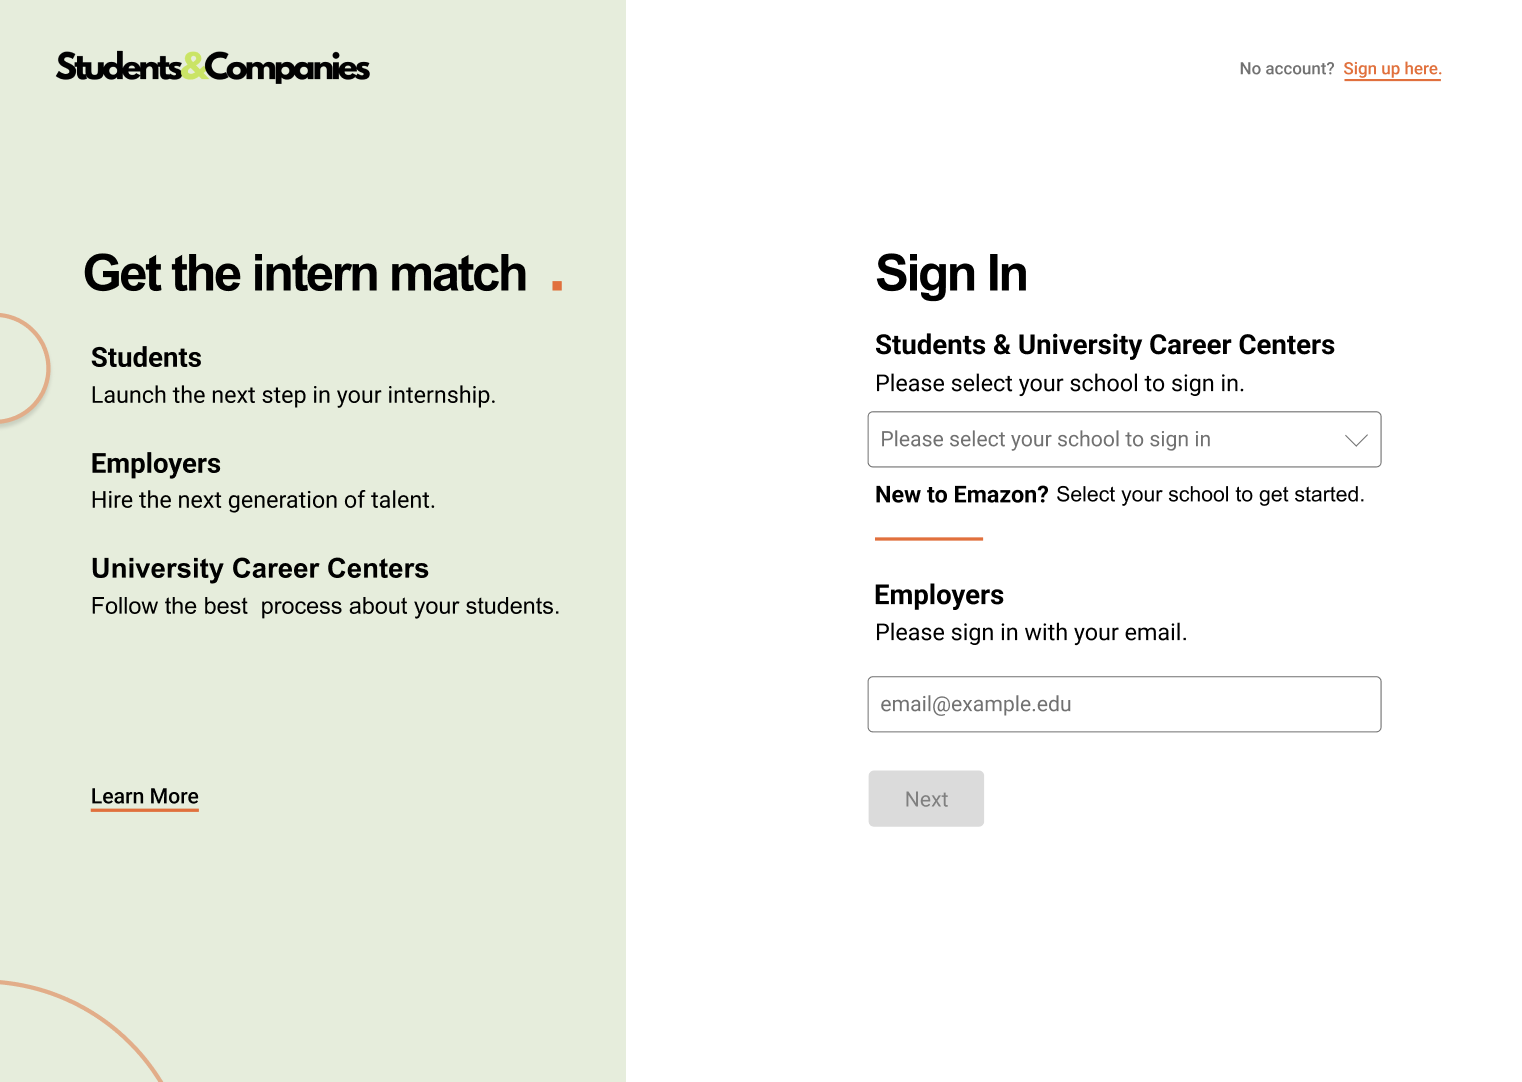
\includegraphics[scale = 0.40]{figures/Sign In.png}
    \caption{Sign In}
     \centering
\end{figure}

\begin{figure}[H]
    \centering
    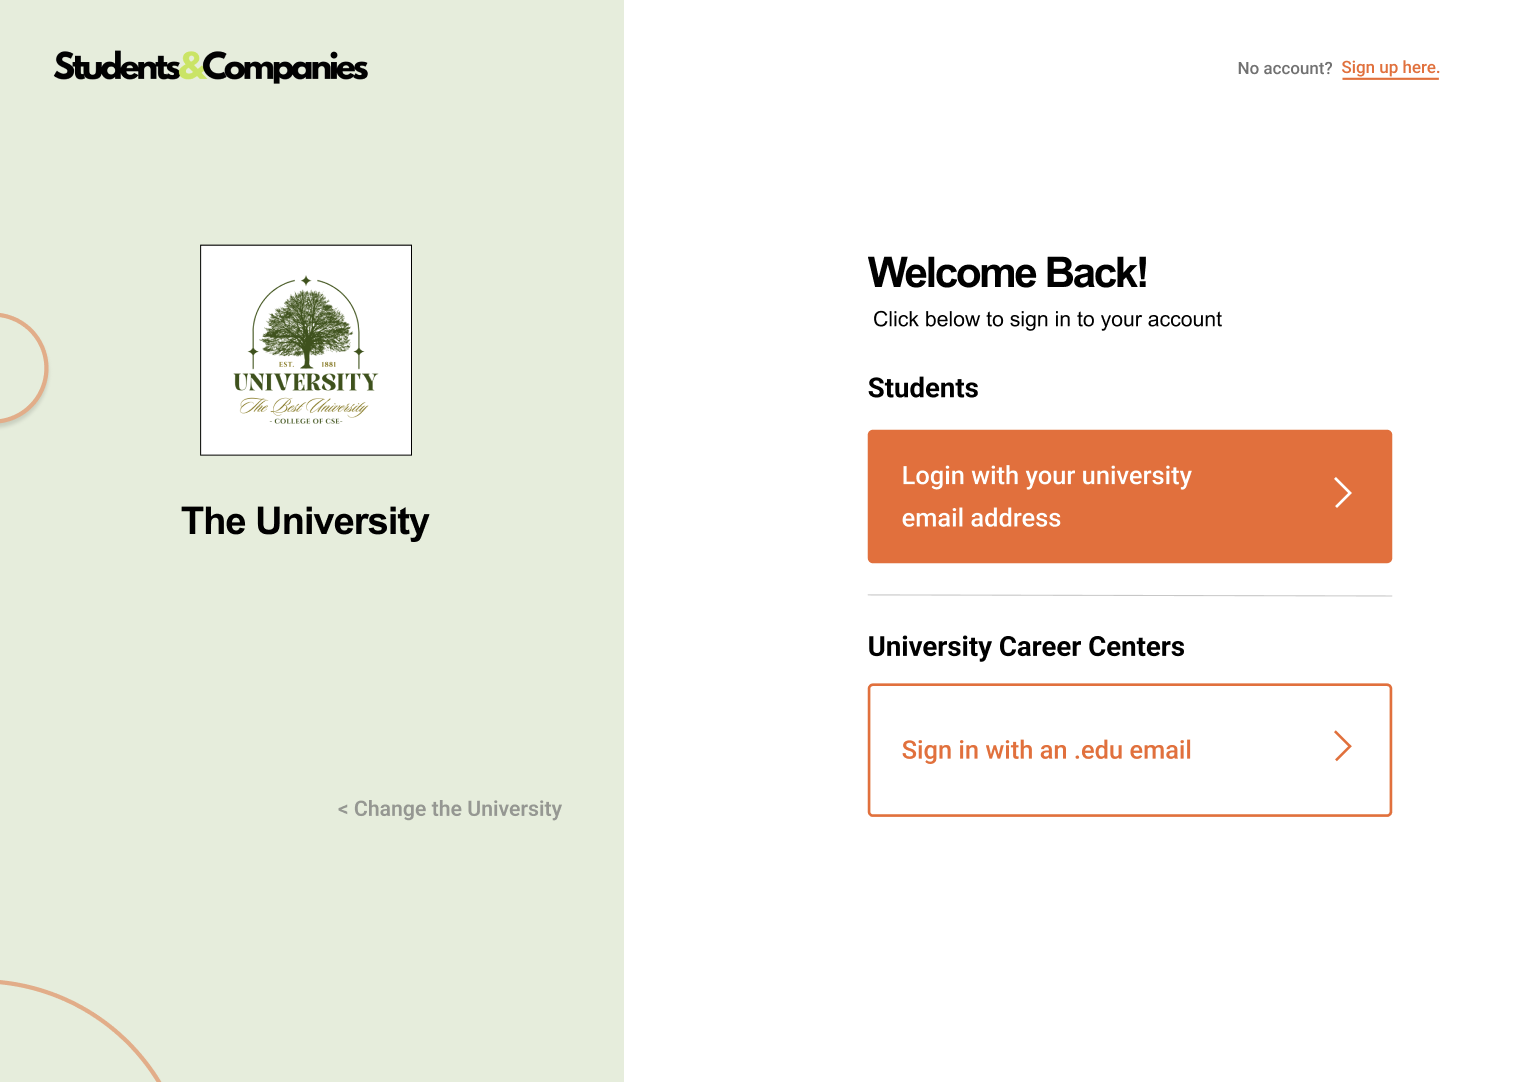
\includegraphics[scale = 0.40]{figures/Student Sign In.png}
    \caption{Student \& University Sign In}
     \centering
\end{figure}
    
\begin{figure}[H]
    \centering
    
\includegraphics[scale = 0.40]{figures/Student Register.png}
    \caption{Student \& University Register}
     \centering
\end{figure}

\begin{figure}[H]
    \centering
    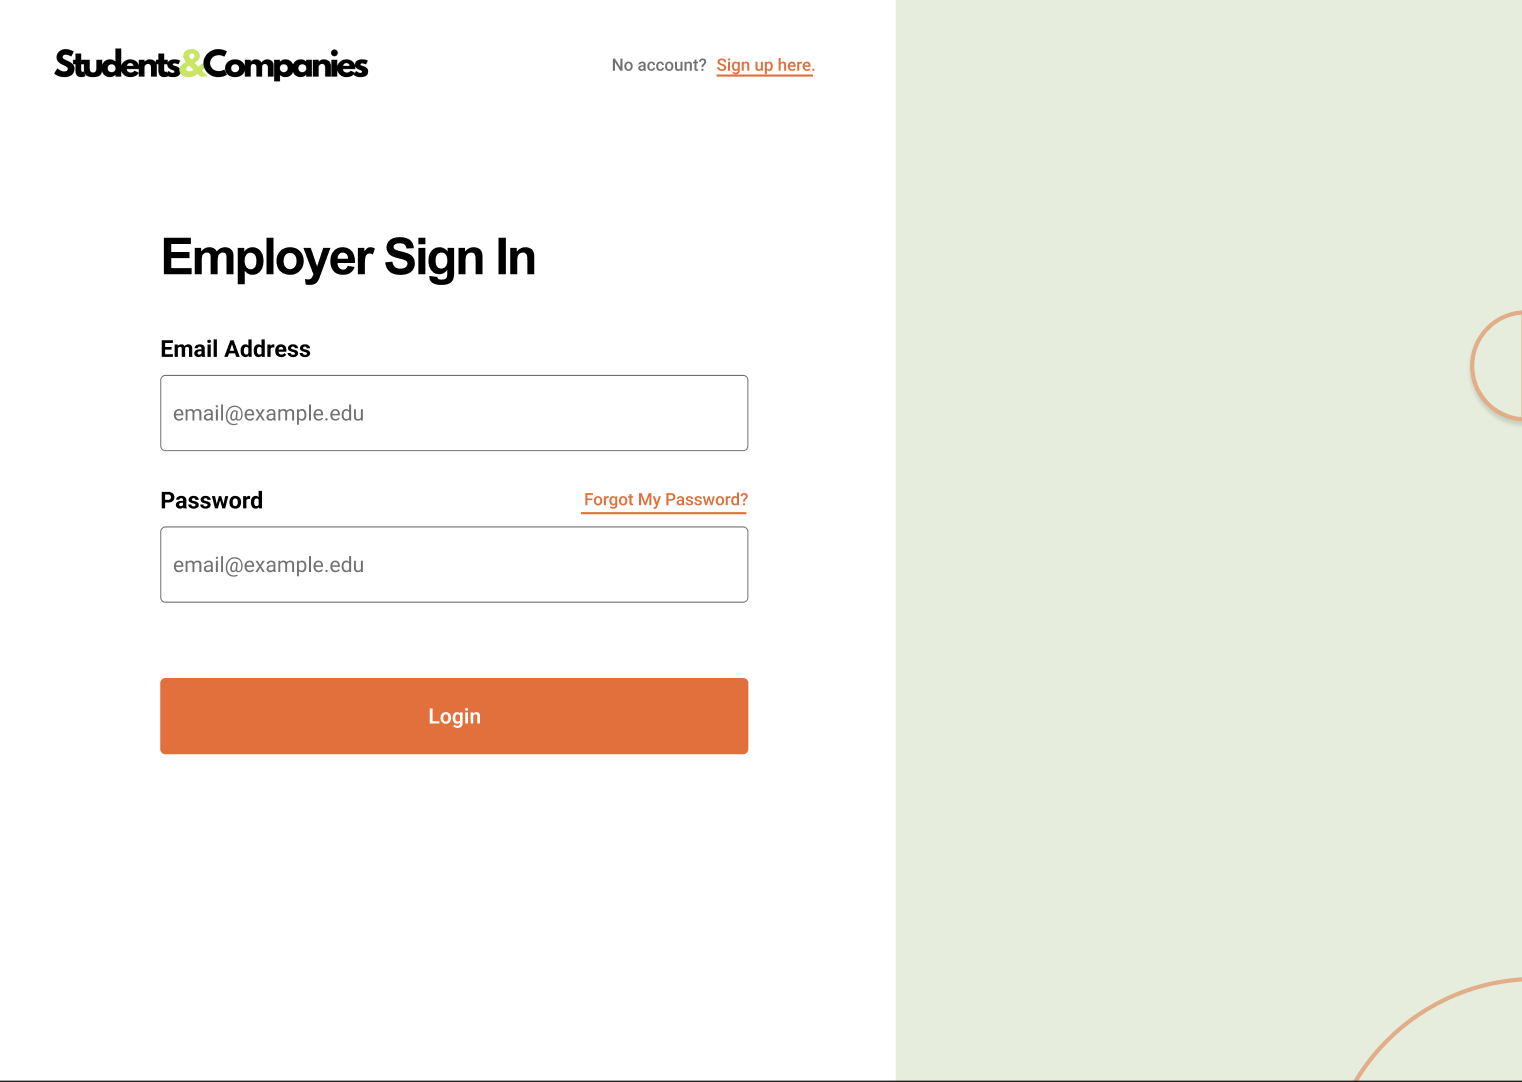
\includegraphics[scale = 0.40]{figures/Employer Sign In.png}
    \caption{Company Sign In}
     \centering
\end{figure}

\begin{figure}[H]
    \centering
    
\includegraphics[scale = 0.40]{figures/Employer Register.png}
    \caption{Company Register}
     \centering
     
\end{figure}
    \begin{figure}[H]
    \centering
    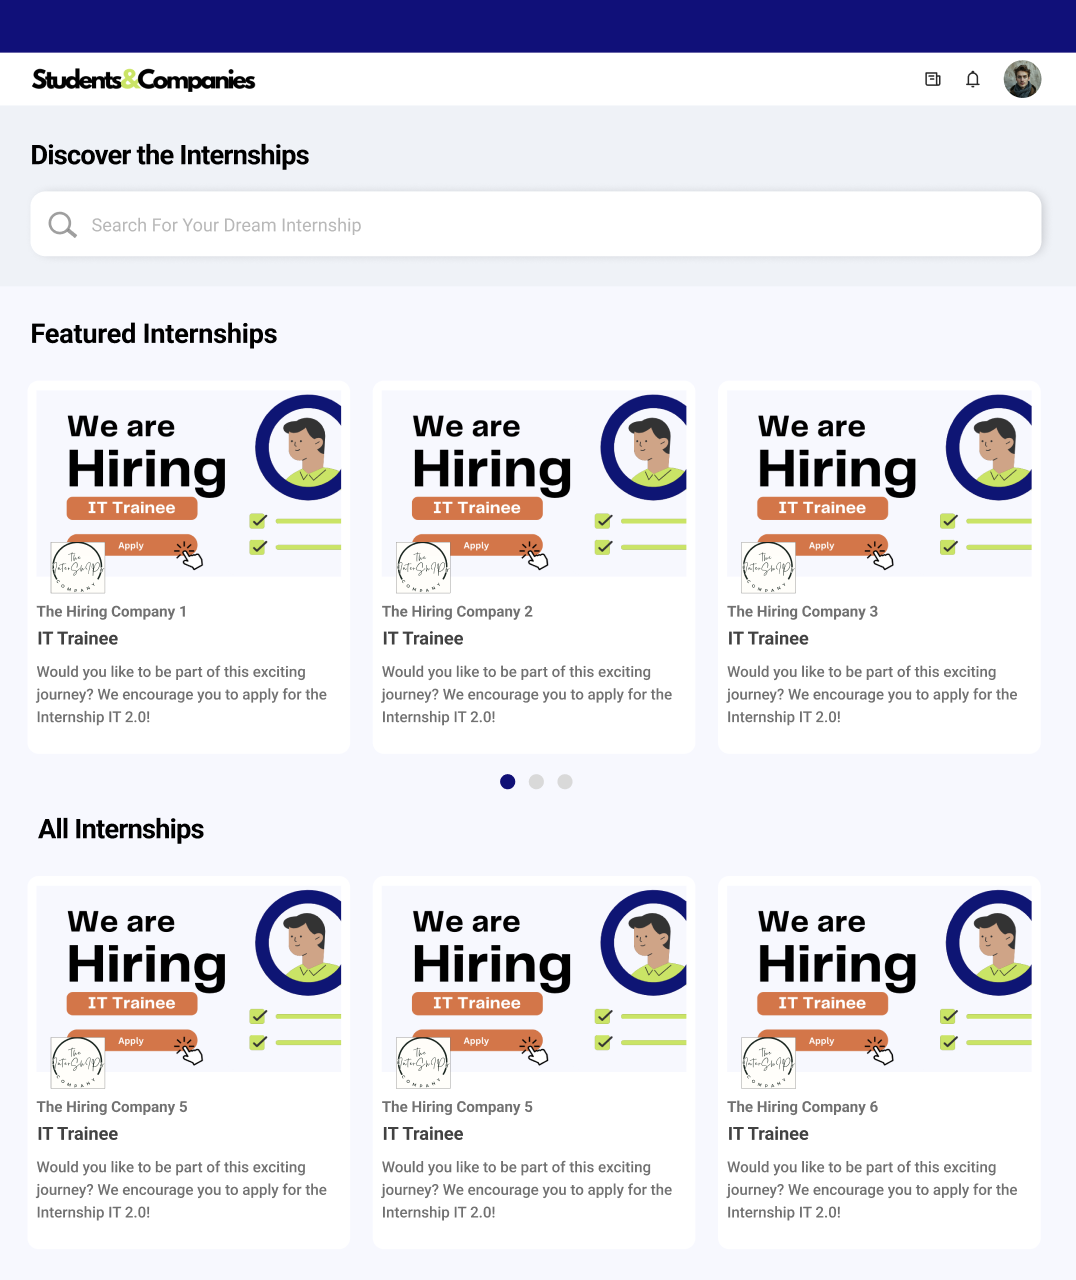
\includegraphics[scale = 0.40]{figures/Home Page1.png}
    \caption{Home Page 1}
     \centering
\end{figure}

\begin{figure}[H]
    \centering
    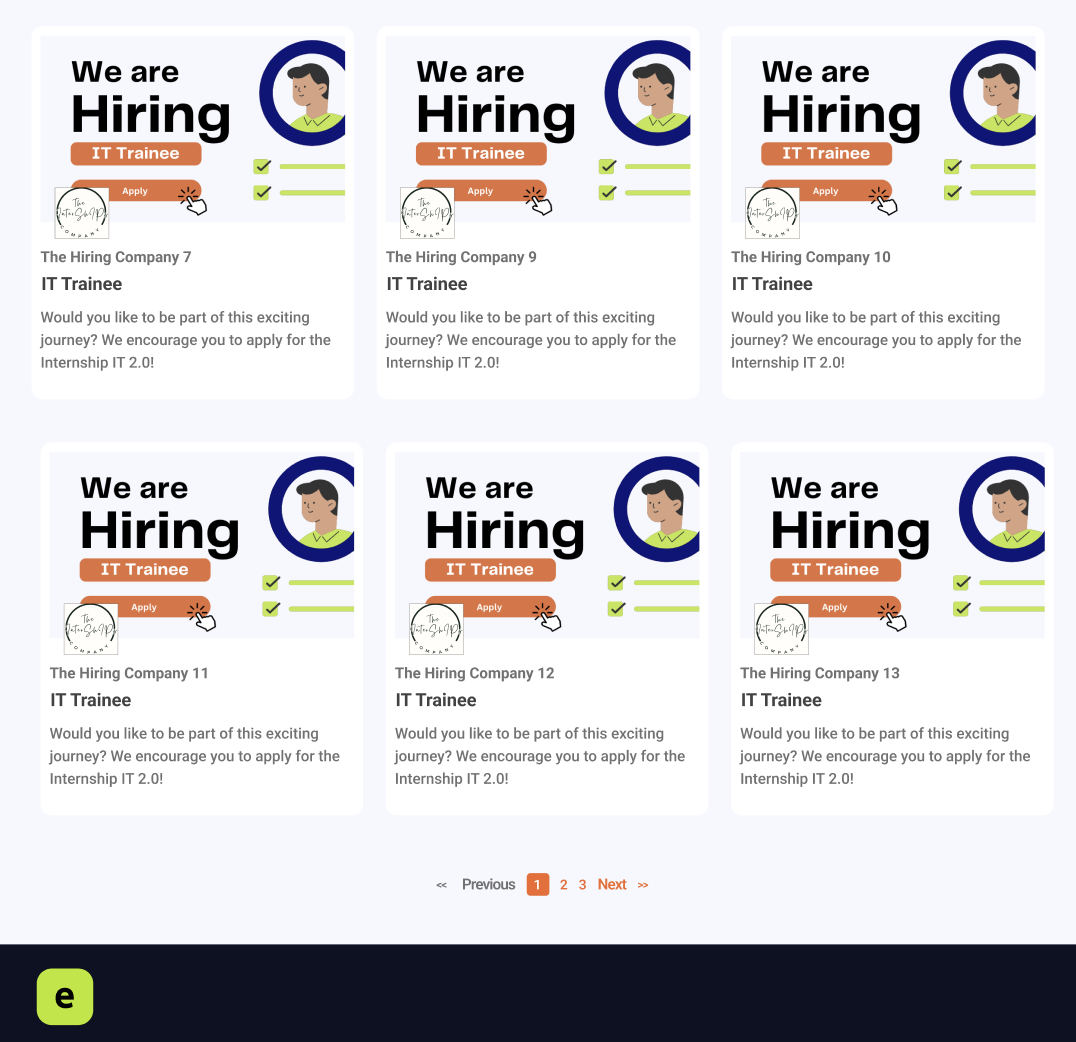
\includegraphics[scale = 0.40]{figures/Home Page 2.png}
    \caption{Home Page 2}
     \centering
\end{figure}

\begin{figure}[H]
    \centering
    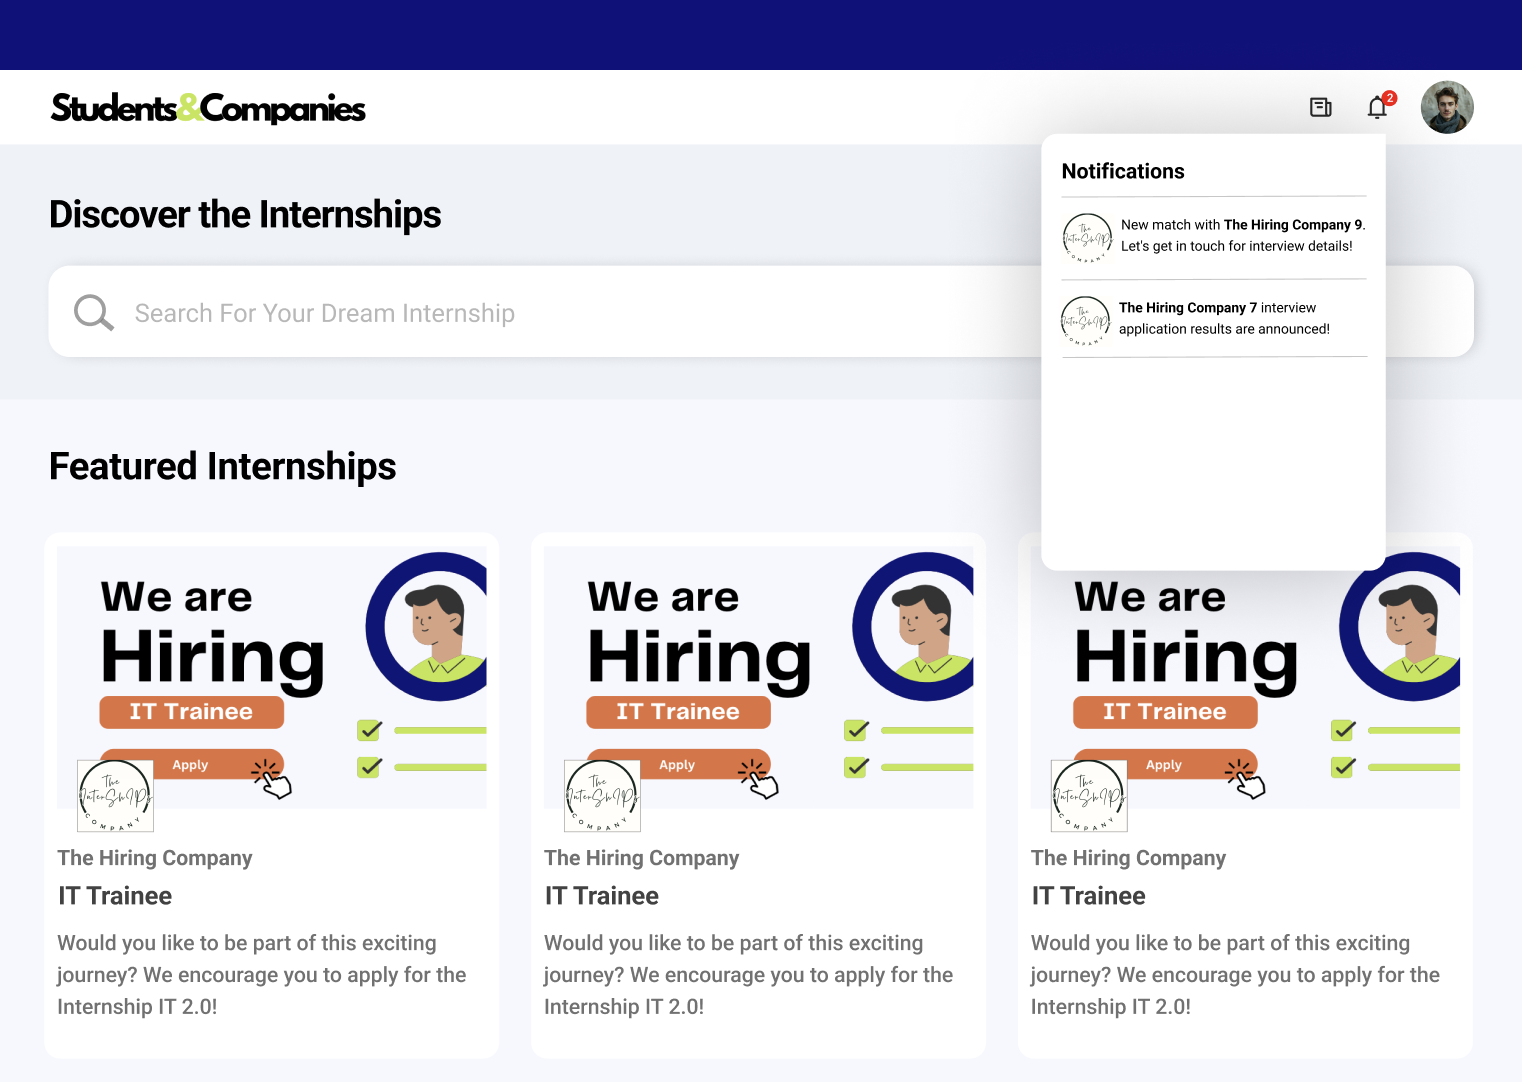
\includegraphics[scale = 0.40]{figures/Notifications.png}
    \caption{Notifications}
     \centering
\end{figure}

\subsubsection{Hardware Interfaces}
    The user, whether a student, university, or company, must use a suitable device to access the system, like a personal computer.
\subsubsection{Software Interfaces}

\subsubsection{Communication Interfaces}
    The system requires a stable internet connection to work properly. This connection is used
    to exchange data between the Users and the central database which contains the information
regarding ongoing Tournaments and Battles
\subsection{Functional Requirements}
\subsubsection{Use Case Diagrams}
\begin{figure}[H]
    \centering
    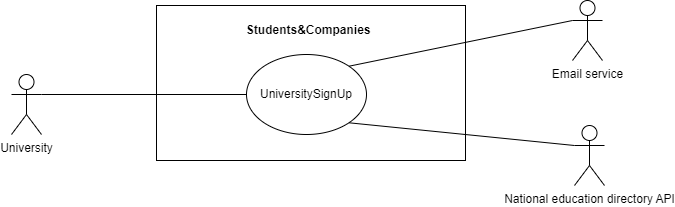
\includegraphics[scale = 0.45]{figures/UniversityLogin.drawio.png}
    \caption{UniversitySignUp}
    \centering
\end{figure}
\begin{figure}[H]
    \centering
    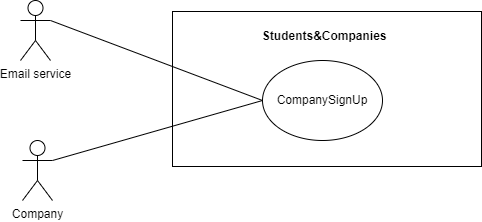
\includegraphics[scale = 0.45]{figures/use_case_1-CompanyLogin.drawio.png}
    \caption{CompanySignUp}
    \centering
\end{figure}
\begin{figure}[H]
    \centering
    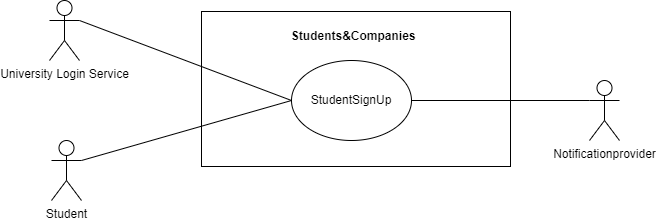
\includegraphics[scale = 0.45]{figures/use_case_1-StudentLogin.drawio.png}
    \caption{StudentSignUp}
    \centering
\end{figure}
\begin{figure}[H]
    \centering
    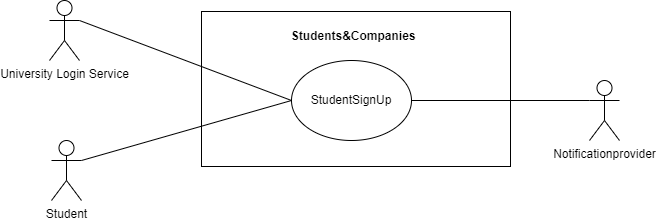
\includegraphics[scale = 0.45]{figures/use_case_1-StudentLogin.drawio.png}
    \caption{StudentLogin}
    \centering
\end{figure}
\begin{figure}[H]
    \centering
    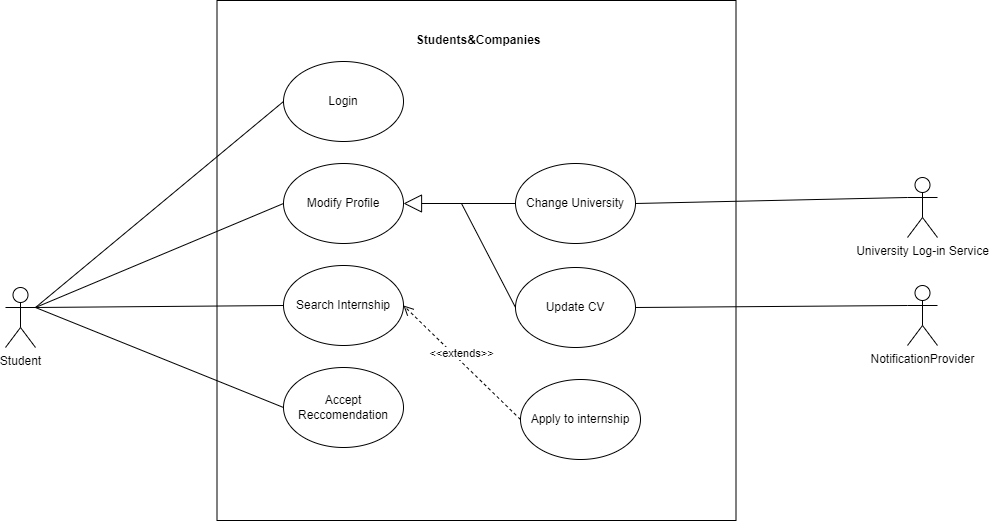
\includegraphics[scale = 0.45]{figures/Student.drawio.png}
    \caption{Student}
    \centering
\end{figure}
\begin{figure}[H]
    \centering
    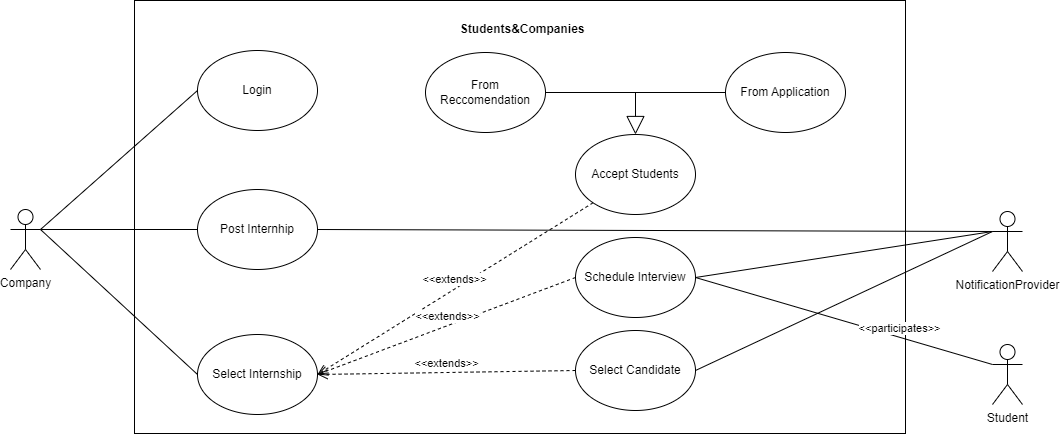
\includegraphics[scale = 0.4]{figures/Company.drawio.png}
    \caption{Company}
    \centering
\end{figure}
\begin{figure}[H]
    \centering
    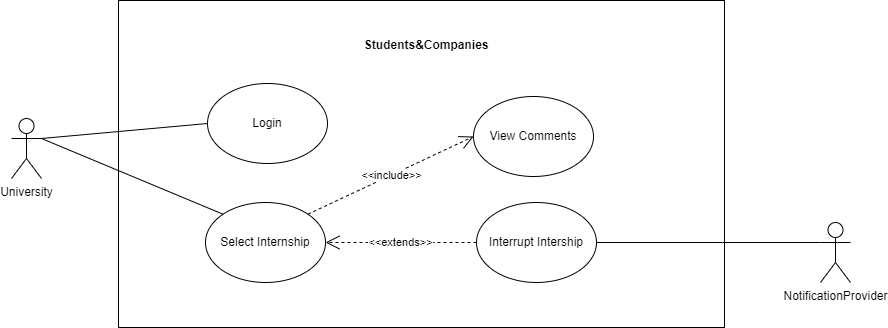
\includegraphics[scale = 0.45]{figures/use_case_1-University.drawio.png}
    \caption{University}
    \centering
\end{figure}
\begin{figure}[H]
    \centering
    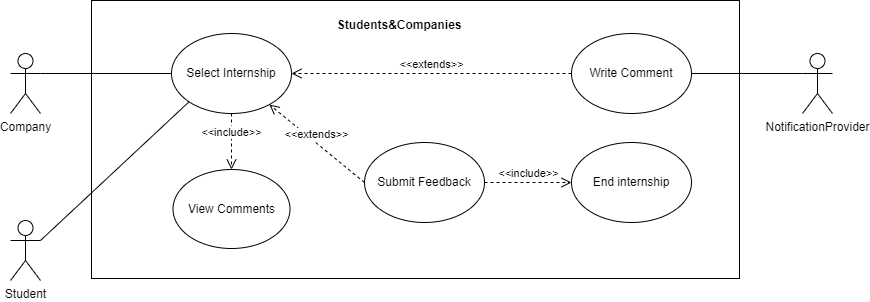
\includegraphics[scale = 0.45]{figures/use_case_1-Student - Company.drawio.png}
    \caption{Internship}
    \centering
\end{figure}
\newpage
\subsubsection{Use cases}
\begin{xltabular}{\textwidth}{| l | X |}
\toprule
\multicolumn{2}{|c|}{StudentsSignUp}\\
\toprule
Participating Actors & Student, EmailService, Students\&Companies\\ [1ex]
\hline
Entry Condition & True\\ [1ex]
\hline
Flow of Events & \begin{itemize}
		      \item 1. The Student opens the “Sign up” page
		      \item 2. Students\&Companies shows the page to sign up
		      \item 3. The Student fills the required informations and clicks “Sign Up” button
		      \item 4. Students\&Companies checks the information provided by the Student
		      \item 5. Students\&Companies registers the Student
                \item 6. Students\&Companies sends confirmation of signup and inform the Student to verify the account
                \item 7. Students\&Companies sends a notification to verify the account through the EmailService
                \item 8. The Student verifies the account
                \item 9. Students\&Companies activates the Student’s account
                \item 10. Students\&Companies sends to the home page 
                \end{itemize} \\ [1ex]
\hline
Exit Condition & The Student successfully signed up and activated his account\\ [1ex]
\hline
Exceptions & The Student was already registered\\ [1ex]
\hline
\end{xltabular}
\begin{figure}[H]
    \centering
    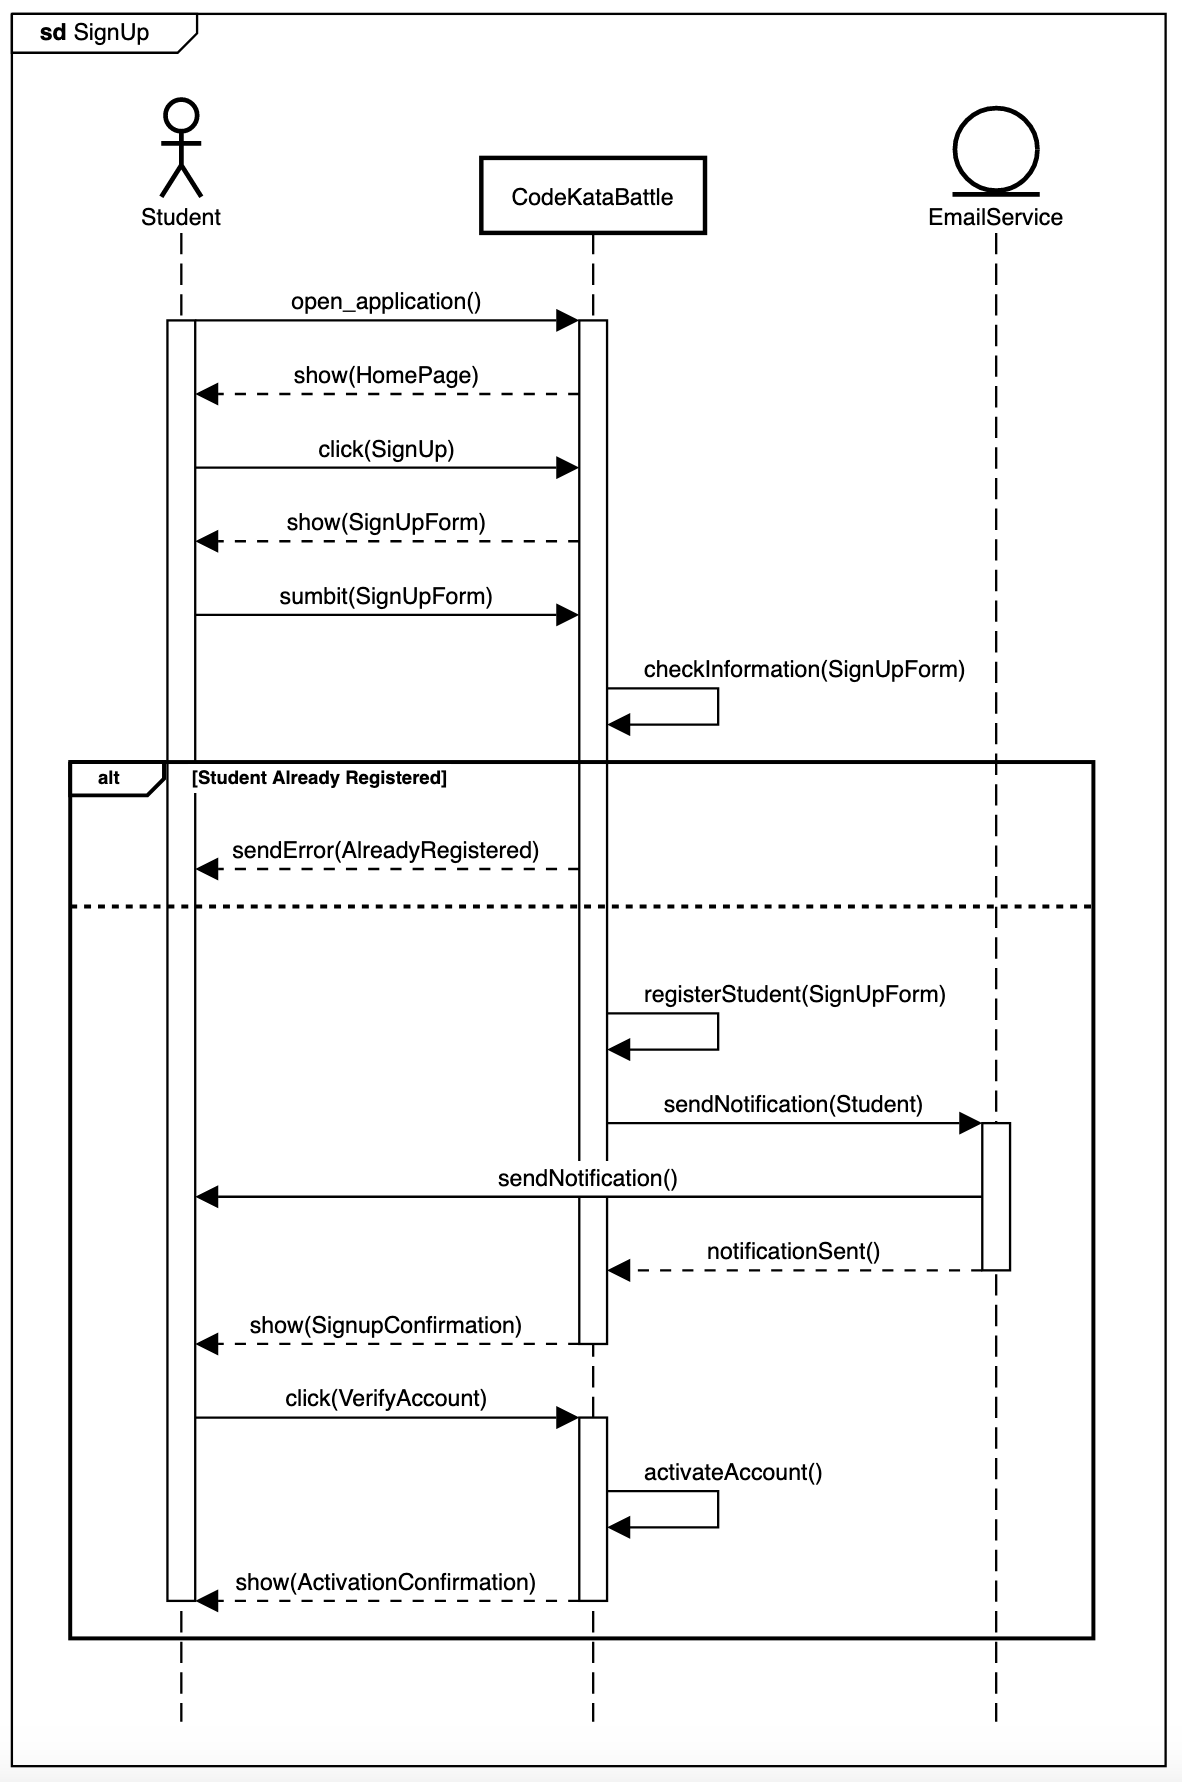
\includegraphics[scale = 0.45]{figures/UseCasesSD/StudentSignUpSeqDiagram.png}\\
\end{figure}

\newpage
\begin{xltabular}{\textwidth}{| l | X |}
\toprule
\multicolumn{2}{|c|}{CompanySignUp}\\
\toprule
Participating Actors & Company, EmailService, Students\&Companies\\ [1ex]
\hline
Entry Condition & True\\ [1ex]
\hline
Flow of Events & \begin{itemize}
		      \item 1. The Company opens the “Sign up” page
		      \item 2. Students\&Companies shows the page to sign up
		      \item 3. The Company fills the required informations and clicks “Require a Company Account” button
		      \item 4. Students\&Companies shows the form to require an Company account
		      \item 5. Students\&Companies registers the Company
                \item 6. Students\&Companies sends confirmation of signup and inform the Company to verify the account
                \item 7. Students\&Companies sends a notification to verify the account through the EmailService
                \item 8. The Company verifies the account
                \item 9. Students\&Companies activates the Company’s account
                \item 10. Students\&Companies sends to the home page 
                \end{itemize} \\ [1ex]
\hline
Exit Condition & The Company successfully signed up and obtained an Company account\\ [1ex]
\hline
Exceptions & The Company was already registered\\ [1ex]
\hline
\end{xltabular}
\begin{figure}[H]
    \centering
    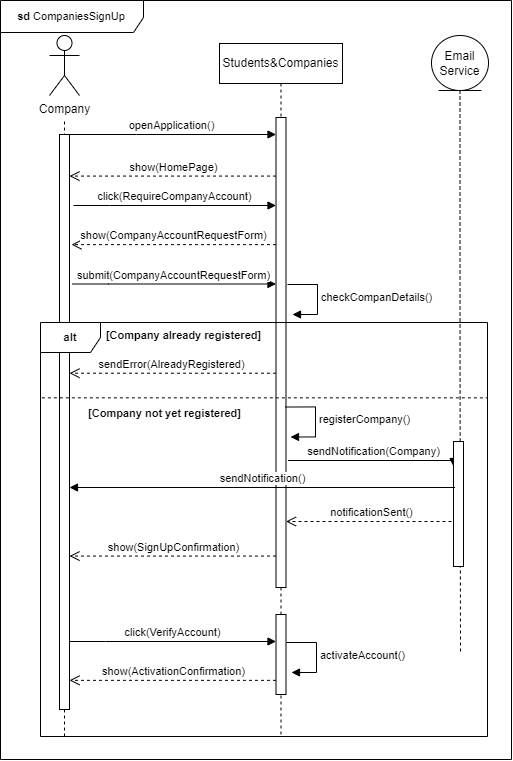
\includegraphics[scale = 0.45]{figures/UseCasesSD/CompanySignUp.drawio.png}\\
\end{figure}
\newpage
\begin{xltabular}{\textwidth}{| l | X |}
\toprule
\multicolumn{2}{|c|}{UniversitySignUp}\\
\toprule
Participating Actors & University, EmailService, National education dictionary
API (NED-API), Students\&Companies\\ [1ex]
\hline
Entry Condition & True\\ [1ex]
\hline
Flow of Events & \begin{itemize}
		      \item 1. The University opens the “Sign up” page
		      \item 2. Students\&Companies shows the page to sign up
		      \item 3. The Company fills the required information and clicks “Require a University Account” button
		      \item 4. Students\&Companies shows the form to require an University account
                \item 5. Students\&Companies check the University existence through he NED-API
		      \item 6. Students\&Companies registers the University
                \item 7. Students\&Companies sends confirmation of sign up and inform the University to verify the account
                \item 8. Students\&Companies sends a notification to verify the account through the EmailService
                \item 9. The University verifies the account
                \item 10. Students\&Companies activates the University’s account
                \item 11. Students\&Companies sends to the home page 
                \end{itemize} \\ [1ex]
\hline
Exit Condition & The University successfully signed up and obtained an University account\\ [1ex]
\hline
Exceptions & \begin{itemize}
                \item The University was already registered
                \item The University does not exist
                \end{itemize} \\ [1ex]
\hline
\end{xltabular}
\begin{figure}[H]
    \centering
    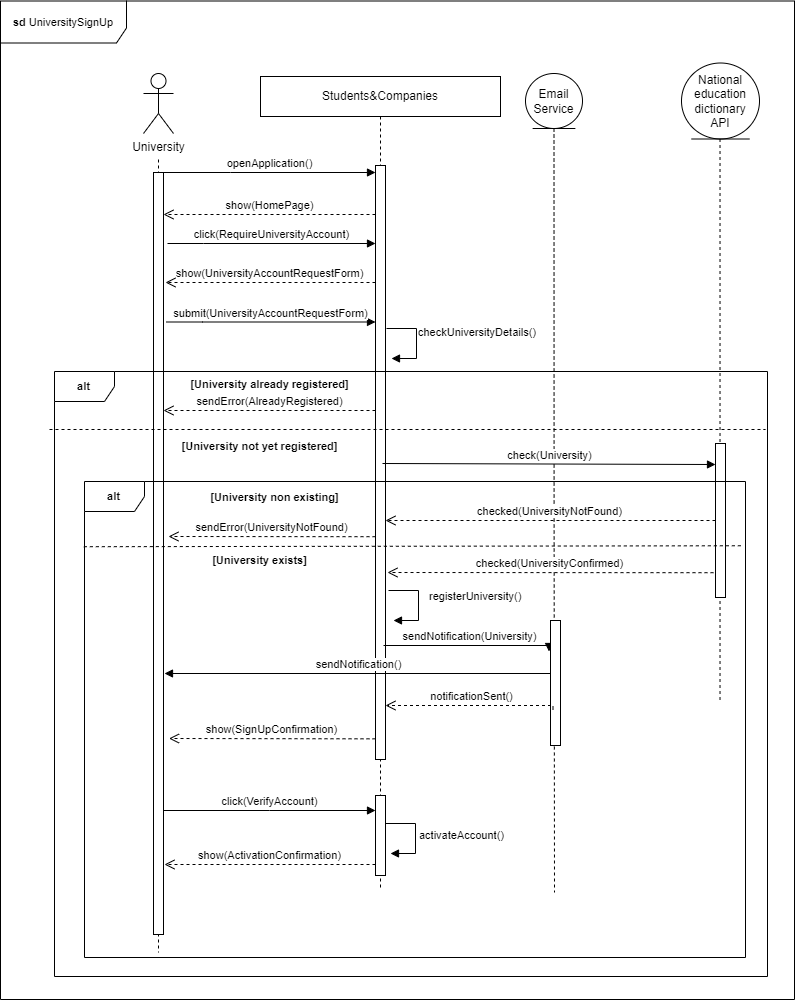
\includegraphics[scale = 0.45]{figures/UseCasesSD/UniversitySignUp.drawio.png}\\
\end{figure}


\newpage
\begin{xltabular}{\textwidth}{| l | X |}
\toprule
\multicolumn{2}{|c|}{UserViewsComments}\\
\toprule
Participating Actors & User (Student, Company, or University), Students\&Companies\\ [1ex]
\hline
Entry Condition & The User is logged into the platform\\ [1ex]
\hline
Flow of Events & \begin{itemize}
		      \item 1. The User navigates to the “View Comments” section
		      \item 2. Students\&Companies retrieves the comments associated with the relevant internship
		      \item 3. Students\&Companies displays the comments to the User
                \end{itemize} \\ [1ex]
\hline
Exit Condition & The User views all comments for the selected internship\\ [1ex]
\hline
Exceptions & No comments are available for the internship\\ [1ex]
\hline
\end{xltabular}


\newpage
\begin{xltabular}{\textwidth}{| l | X |}
\toprule
\multicolumn{2}{|c|}{UserWritesComment}\\
\toprule
Participating Actors & User (Student or Company), Students\&Companies\\ [1ex]
\hline
Entry Condition & The User is logged into the platform\\ [1ex]
\hline
Flow of Events & \begin{itemize}
		      \item 1. The User navigates to the “Write Comment” section
		      \item 2. Students\&Companies displays the comment input form
		      \item 3. The User writes the comment and submits it
		      \item 4. Students\&Companies validates the input and saves the comment
		      \item 5. Students\&Companies notifies the relevant User (Student or Company) of the new comment
                \end{itemize} \\ [1ex]
\hline
Exit Condition & The comment is successfully saved and notified to the other party\\ [1ex]
\hline
Exceptions & The comment is invalid (e.g., empty or contains restricted content)\\ [1ex]
\hline
\end{xltabular}
\newpage

\begin{xltabular}{\textwidth}{| l | X |}
\toprule
\multicolumn{2}{|c|}{UniversityInterruptsInternship}\\
\toprule
Participating Actors & University, Students\&Companies\\ [1ex]
\hline
Entry Condition & The University is logged into the platform and identifies an issue with the internship\\ [1ex]
\hline
Flow of Events & \begin{itemize}
		      \item 1. The University navigates to the “Interrupt Internship” section
		      \item 2. Students\&Companies displays a list of ongoing internships
		      \item 3. The University selects the internship to be interrupted and provides a justification
		      \item 4. Students\&Companies interrupts the internship and notifies the Student and the Company
                \end{itemize} \\ [1ex]
\hline
Exit Condition & The internship is interrupted and both parties are notified\\ [1ex]
\hline
Exceptions & The University cannot interrupt an internship already completed\\ [1ex]
\hline
\end{xltabular}
\newpage

\begin{xltabular}{\textwidth}{| l | X |}
\toprule
\multicolumn{2}{|c|}{UserSubmitsFeedback}\\
\toprule
Participating Actors & User (Student or Company), Students\&Companies\\ [1ex]
\hline
Entry Condition & The User is logged into the platform and the internship is near completion\\ [1ex]
\hline
Flow of Events & \begin{itemize}
		      \item 1. The User navigates to the “Submit Feedback” section
		      \item 2. Students\&Companies displays the feedback input form
		      \item 3. The User fills out and submits the feedback form
		      \item 4. Students\&Companies saves the feedback and marks the internship as completed for the submitting User
		      \item 5. If both parties have submitted feedback, Students\&Companies marks the internship as fully completed
                \end{itemize} \\ [1ex]
\hline
Exit Condition & The feedback is successfully saved, and the internship is marked as completed for the submitting User\\ [1ex]
\hline
Exceptions & Feedback submission fails due to invalid input or technical issues\\ [1ex]
\hline
\end{xltabular}
\newpage

\begin{xltabular}{\textwidth}{| l | X |}
\toprule
\multicolumn{2}{|c|}{UserLogsIn}\\
\toprule
Participating Actors & User (Student, Company, or University), Students\&Companies\\ [1ex]
\hline
Entry Condition & The User has an account on the platform\\ [1ex]
\hline
Flow of Events & \begin{itemize}
		      \item 1. The User opens the login page
		      \item 2. Students\&Companies displays the login form
		      \item 3. The User enters their credentials and submits the form
		      \item 4. Students\&Companies validates the credentials
		      \item 5. If valid, Students\&Companies grants access and redirects the User to their dashboard
                \end{itemize} \\ [1ex]
\hline
Exit Condition & The User successfully logs in and accesses their dashboard\\ [1ex]
\hline
Exceptions & Invalid credentials or account locked due to too many failed attempts\\ [1ex]
\hline
\end{xltabular}
\newpage

\begin{xltabular}{\textwidth}{| l | X |}
\toprule
\multicolumn{2}{|c|}{StudentChangesUniversity}\\
\toprule
Participating Actors & Student, Students\&Companies\\ [1ex]
\hline
Entry Condition & The Student is logged in and has an active account\\ [1ex]
\hline
Flow of Events & \begin{itemize}
		      \item 1. The Student navigates to the “Profile” section
		      \item 2. Students\&Companies displays the current university information
		      \item 3. The Student selects the option to change the university and provides the new details
		      \item 4. Students\&Companies validates and updates the university information
                \end{itemize} \\ [1ex]
\hline
Exit Condition & The Student's university information is successfully updated\\ [1ex]
\hline
Exceptions & Invalid or incomplete university information provided\\ [1ex]
\hline
\end{xltabular}
\newpage

\begin{xltabular}{\textwidth}{| l | X |}
\toprule
\multicolumn{2}{|c|}{StudentUpdatesCV}\\
\toprule
Participating Actors & Student, Students\&Companies\\ [1ex]
\hline
Entry Condition & The Student is logged in and has uploaded a CV in the past\\ [1ex]
\hline
Flow of Events & \begin{itemize}
		      \item 1. The Student navigates to the “Update CV” section
		      \item 2. Students\&Companies displays the current CV and an option to upload a new one
		      \item 3. The Student uploads a new CV file
		      \item 4. Students\&Companies validates the file format and replaces the old CV
                \end{itemize} \\ [1ex]
\hline
Exit Condition & The Student's CV is successfully updated\\ [1ex]
\hline
Exceptions & File upload fails due to incorrect format or size\\ [1ex]
\hline
\end{xltabular}
\newpage

\begin{xltabular}{\textwidth}{| l | X |}
\toprule
\multicolumn{2}{|c|}{CompanyPostsInternship}\\
\toprule
Participating Actors & Company, Students\&Companies\\ [1ex]
\hline
Entry Condition & The Company is logged in\\ [1ex]
\hline
Flow of Events & \begin{itemize}
		      \item 1. The Company navigates to the “Post Internship” section
		      \item 2. Students\&Companies displays the internship creation form
		      \item 3. The Company fills out the form with internship details and submits it
		      \item 4. Students\&Companies validates the information and publishes the internship
                \end{itemize} \\ [1ex]
\hline
Exit Condition & The internship is successfully posted and visible to Students\\ [1ex]
\hline
Exceptions & Invalid or incomplete internship details provided\\ [1ex]
\hline
\end{xltabular}
\newpage

\begin{xltabular}{\textwidth}{| l | X |}
\toprule
\multicolumn{2}{|c|}{StudentSearchesForInternship}\\
\toprule
Participating Actors & Student, Students\&Companies\\ [1ex]
\hline
Entry Condition & The Student is logged in\\ [1ex]
\hline
Flow of Events & \begin{itemize}
		      \item 1. The Student navigates to the “Search Internship” section
		      \item 2. Students\&Companies displays filters and search options
		      \item 3. The Student enters criteria and performs a search
		      \item 4. Students\&Companies retrieves and displays matching internships
                \end{itemize} \\ [1ex]
\hline
Exit Condition & The Student views a list of internships matching their criteria\\ [1ex]
\hline
Exceptions & No internships match the search criteria\\ [1ex]
\hline
\end{xltabular}
\newpage

\begin{xltabular}{\textwidth}{| l | X |}
\toprule
\multicolumn{2}{|c|}{StudentAppliesToInternship}\\
\toprule
Participating Actors & Student, Students\&Companies\\ [1ex]
\hline
Entry Condition & The Student is logged in and has found an internship\\ [1ex]
\hline
Flow of Events & \begin{itemize}
		      \item 1. The Student selects an internship to apply for
		      \item 2. Students\&Companies displays the application form
		      \item 3. The Student completes and submits the form
		      \item 4. Students\&Companies saves the application and notifies the Company
                \end{itemize} \\ [1ex]
\hline
Exit Condition & The application is successfully submitted and the Company is notified\\ [1ex]
\hline
Exceptions & The internship application deadline has passed\\ [1ex]
\hline
\end{xltabular}
\newpage

\begin{xltabular}{\textwidth}{| l | X |}
\toprule
\multicolumn{2}{|c|}{UserSelectsInternship}\\
\toprule
Participating Actors & User (Student, Company, or University), Students\&Companies\\ [1ex]
\hline
Entry Condition & The User is logged in\\ [1ex]
\hline
Flow of Events & \begin{itemize}
		      \item 1. The User navigates to a list of internships
		      \item 2. Students\&Companies displays internship details
		      \item 3. The User selects an internship from the list
		      \item 4. Students\&Companies highlights or saves the selected internship for the User
                \end{itemize} \\ [1ex]
\hline
Exit Condition & The User successfully selects an internship\\ [1ex]
\hline
Exceptions & The internship is no longer available\\ [1ex]
\hline
\end{xltabular}
\newpage

\begin{xltabular}{\textwidth}{| l | X |}
\toprule
\multicolumn{2}{|c|}{UserAcceptsRecommendation}\\
\toprule
Participating Actors & User (Student or Company), Students\&Companies\\ [1ex]
\hline
Entry Condition & The User has received a recommendation\\ [1ex]
\hline
Flow of Events & \begin{itemize}
		      \item 1. The User navigates to the “Recommendations” section
		      \item 2. Students\&Companies displays recommended internships or candidates
		      \item 3. The User reviews and accepts a recommendation
		      \item 4. Students\&Companies saves the acceptance and notifies the other party
                \end{itemize} \\ [1ex]
\hline
Exit Condition & The recommendation is accepted and the other party is notified\\ [1ex]
\hline
Exceptions & The recommended internship or candidate is no longer available\\ [1ex]
\hline
\end{xltabular}
\newpage

\begin{xltabular}{\textwidth}{| l | X |}
\toprule
\multicolumn{2}{|c|}{CompanyAcceptsApplication}\\
\toprule
Participating Actors & Company, Students\&Companies\\ [1ex]
\hline
Entry Condition & The Company has received applications from Students\\ [1ex]
\hline
Flow of Events & \begin{itemize}
		      \item 1. The Company reviews the applications
		      \item 2. Students\&Companies displays a list of applicants
		      \item 3. The Company selects a Student and accepts the application
		      \item 4. Students\&Companies updates the status and notifies the Student
                \end{itemize} \\ [1ex]
\hline
Exit Condition & The application is accepted, and the Student is notified\\ [1ex]
\hline
Exceptions & The Company has already filled the internship position\\ [1ex]
\hline
\end{xltabular}
\newpage

\begin{xltabular}{\textwidth}{| l | X |}
\toprule
\multicolumn{2}{|c|}{CompanySchedulesInterview}\\
\toprule
Participating Actors & Company, Students\&Companies\\ [1ex]
\hline
Entry Condition & The deadline for internship applications has passed, and the Company has accepted applications\\ [1ex]
\hline
Flow of Events & \begin{itemize}
		      \item 1. The Company navigates to the “Schedule Interview” section
		      \item 2. Students\&Companies displays a list of accepted candidates
		      \item 3. The Company selects a candidate and schedules the interview date
		      \item 4. Students\&Companies sends an interview invitation to the selected candidate
                \end{itemize} \\ [1ex]
\hline
Exit Condition & The interview is successfully scheduled and the candidate is notified\\ [1ex]
\hline
Exceptions & No available candidates or interview slots\\ [1ex]
\hline
\end{xltabular}
\newpage

\subsubsection{Mapping}
\begin{center}
    \begin{tabular}{|C{3cm}|p{10cm}|}
    \hline
    \multicolumn{2}{|c|}{\parbox{13cm}{G1: Allows registered companies to post and advertise the available internships that they offer.}} \\
    \hline
    \centering R1 & The system must allow a student who wants to register to sign up. \\ 
    \hline
    \centering R2 & The system must allow a company who wants to register to sign up. \\ 
    \hline
    \centering R4 & The system must allow registered users to sign in using their credentials. \\ 
    \hline
    \centering R7 & The system must allow registered students to enter information from their CV to complete their profiles. \\ 
    \hline
    \centering R8 & The system must allow registered companies to post internship advertisements. \\ 
    \hline
    \centering R9 & The system must allow companies to review students' CVs and select candidates who meet their internship requirements. \\ 
    \hline
    \centering R10 & The system must allow students to review internship advertisements and select them if they wish to apply. \\ 
    \hline
    \centering R12 & The system must notify students when there are updates regarding the internships at the companies in their favorites that they wish to apply for. \\ 
    \hline
    \centering R16 & The system must recommend a student and a company profile to each other and allow them to review whether the company has an active internship position and if the profiles could attract each other's interest. \\ 
    \hline
    \centering R21 & The system must notify students when there are updates regarding the results of the internships they have applied for. \\ 
    \hline
    \centering R23 & The system must notify students about deadlines for accepting internship offers. \\ 
    \hline
    \centering R25 & The system must allow students to view all details about the internships they have applied for, such as completion status, rejections, and deadlines. \\ 
    \hline
    \centering D5 & All universities are registered before their students. \\ 
    \hline
    \end{tabular}
\end{center}


    
\begin{center}
    \begin{tabular}{|C{3cm}|p{10cm}|}
    \hline
    \multicolumn{2}{|c|}{\parbox{13cm}{G2: Allows registered students to proactively and autonomously search and apply internships.}} \\
    \hline
    \centering R1 & The system must allow a student who wants to register to sign up. \\ 
    \hline
    \centering R4 & The system must allow registered users to sign in using their credentials. \\ 
    \hline
    \centering R7 & The system must allow registered students to enter information from their CV to complete their profiles. \\ 
    \hline
    \centering R11 & The system must allow students to manually search for internship opportunities and apply for them. \\ 
    \hline
    \centering D5 & All universities are registered before their students. \\ 
    \hline
    \end{tabular}
\end{center}


\begin{center}
    \begin{tabular}{|C{3cm}|p{10cm}|}
    \hline
    \multicolumn{2}{|c|}{\parbox{13cm}{G3: Helps registered students and registered companies by suggesting them appealing templates for their CVs and internship projects drafts.}} \\
    \hline
    \centering R1 & The system must allow a student who wants to register to sign up. \\ 
    \hline
    \centering R2 & The system must allow a company who wants to register to sign up. \\ 
    \hline
    \centering R4 & The system must allow registered users to sign in using their credentials. \\ 
    \hline
    \centering R6 & The system must be able to send notifications to all users. \\ 
    \hline
    \centering R7 & The system must allow registered students to enter information from their CV to complete their profiles. \\ 
    \hline
    \centering R8 & The system must allow registered companies to post internship advertisements. \\ 
    \hline
    \centering R18 & The system must allow companies to evaluate students during the internship process and provide feedback on their CVs. \\ 
    \hline
    \centering R20 & The system must provide suggestions to users for improving their profiles based on feedback. \\ 
    \hline
    \centering D5 & All universities are registered before their students. \\ 
    \hline
    \end{tabular}
\end{center}


\begin{center}
    \begin{tabular}{|C{3cm}|p{10cm}|}
    \hline
    \multicolumn{2}{|c|}{\parbox{13cm}{G4: Allows a registered student to be recommended a list of advertised internships that might be of interest to him/her with respect to: his/her uploaded CV, the internships projects, and users' feedbacks.}} \\
    \hline
    \centering R1 & The system must allow a student who wants to register to sign up. \\ 
    \hline
    \centering R2 & The system must allow a company who wants to register to sign up. \\ 
    \hline
    \centering R3 & The system must allow a university who wants to register to sign up. \\ 
    \hline
    \centering R4 & The system must allow registered users to sign in using their credentials. \\ 
    \hline
    \centering R6 & The system must be able to send notifications to all users. \\ 
    \hline
    \centering R7 & The system must allow registered students to enter information from their CV to complete their profiles. \\ 
    \hline
    \centering R8 & The system must allow registered companies to post internship advertisements. \\ 
    \hline
    \centering D5 & All universities are registered before their students. \\ 
    \hline
    \end{tabular}
\end{center}

\begin{center}
    \begin{tabular}{|C{3cm}|p{10cm}|}
    \hline
    \multicolumn{2}{|c|}{\parbox{13cm}{G5: Allows a registered company to be recommended a list of registered students who might be of interest for one of its advertised internships with respect to: their uploaded CVs, the internship project and users' feedbacks.}} \\
    \hline
    \centering R1 & The system must allow a student who wants to register to sign up. \\ 
    \hline
    \centering R2 & The system must allow a company who wants to register to sign up. \\ 
    \hline
    \centering R3 & The system must allow a university who wants to register to sign up. \\ 
    \hline
    \centering R4 & The system must allow registered users to sign in using their credentials. \\ 
    \hline
    \centering R7 & The system must allow registered students to enter information from their CV to complete their profiles. \\ 
    \hline
    \centering R8 & The system must allow registered companies to post internship advertisements. \\ 
    \hline
    \centering D5 & All universities are registered before their students. \\ 
    \hline
    \end{tabular}
\end{center}

\begin{center}
    \begin{tabular}{|C{3cm}|p{10cm}|}
    \hline
    \multicolumn{2}{|c|}{\parbox{13cm}{G6: Allows a registered company to view the list of all the students who applied to one of its advertised internships grouped by the internship they applied to.}} \\
    \hline
    \centering D5 & All universities are registered before their students. \\ 
    \hline
    \end{tabular}
\end{center}

\begin{center}
    \begin{tabular}{|C{3cm}|p{10cm}|}
    \hline
    \multicolumn{2}{|c|}{\parbox{13cm}{G7: Allows a registered student to access the list of internships that he/she has applied for and the ones that he/she has accepted, along with deadlines and other important details.}} \\
    \hline
    \centering R4 & The system must allow registered users to sign in using their credentials. \\ 
    \hline
    \centering R7 & The system must allow registered students to enter information from their CV to complete their profiles. \\ 
    \hline
    \centering R10 & The system must allow students to review internship advertisements and select them if they wish to apply. \\ 
    \hline
    \centering R25 & The system must allow students to view all details about the internships they have applied for, such as completion status, rejections, and deadlines. \\ 
    \hline
    \centering D5 & All universities are registered before their students. \\ 
    \hline
    \end{tabular}
\end{center}

\begin{center}
    \begin{tabular}{|C{3cm}|p{10cm}|}
    \hline
    \multicolumn{2}{|c|}{\parbox{13cm}{G8: Allows a registered company to access the list of students that applied to its internships and the status of each student's application (rejected, selected, etc.).}} \\
    \hline
    \centering R4 & The system must allow registered users to sign in using their credentials. \\ 
    \hline
    \centering R8 & The system must allow registered companies to post internship advertisements. \\ 
    \hline
    \centering R9 & The system must allow companies to review students' CVs and select candidates who meet their internship requirements. \\ 
    \hline
    \centering R16 & The system must recommend a student and a company profile to each other and allow them to review whether the company has an active internship position and if the profiles could attract each other's interest. \\ 
    \hline
    \centering D5 & All universities are registered before their students. \\ 
    \hline
    \end{tabular}
\end{center}

\begin{center}
    \begin{tabular}{|C{3cm}|p{10cm}|}
    \hline
    \multicolumn{2}{|c|}{\parbox{13cm}{G9: Allows a registered student to view a list of available internships sorted by company, internship description, deadline, and application status.}} \\
    \hline
    \centering R4 & The system must allow registered users to sign in using their credentials. \\ 
    \hline
    \centering R7 & The system must allow registered students to enter information from their CV to complete their profiles. \\ 
    \hline
    \centering R10 & The system must allow students to review internship advertisements and select them if they wish to apply. \\ 
    \hline
    \centering R12 & The system must notify students when there are updates regarding the internships at the companies in their favorites that they wish to apply for. \\ 
    \hline
    \centering D5 & All universities are registered before their students. \\ 
    \hline
    \end{tabular}
\end{center}

\begin{center}
    \begin{tabular}{|C{3cm}|p{10cm}|}
    \hline
    \multicolumn{2}{|c|}{\parbox{13cm}{G10: Allows a registered company to track and update the application status of students applying to its internships.}} \\
    \hline
    \centering R4 & The system must allow registered users to sign in using their credentials. \\ 
    \hline
    \centering R8 & The system must allow registered companies to post internship advertisements. \\ 
    \hline
    \centering R9 & The system must allow companies to review students' CVs and select candidates who meet their internship requirements. \\ 
    \hline
    \centering R15 & The system must allow companies to provide feedback to students regarding their application status. \\ 
    \hline
    \centering D5 & All universities are registered before their students. \\ 
    \hline
    \end{tabular}
\end{center}

\begin{center}
    \begin{tabular}{|C{3cm}|p{10cm}|}
    \hline
    \multicolumn{2}{|c|}{\parbox{13cm}{G11: Allows registered students and companies to communicate with each other regarding internship applications and statuses.}} \\
    \hline
    \centering R4 & The system must allow registered users to sign in using their credentials. \\ 
    \hline
    \centering R8 & The system must allow registered companies to post internship advertisements. \\ 
    \hline
    \centering R10 & The system must allow students to review internship advertisements and select them if they wish to apply. \\ 
    \hline
    \centering R12 & The system must notify students when there are updates regarding the internships at the companies in their favorites that they wish to apply for. \\ 
    \hline
    \centering R14 & The system must allow students to contact companies regarding the internships they applied for. \\ 
    \hline
    \centering D5 & All universities are registered before their students. \\ 
    \hline
    \end{tabular}
\end{center}



	
	

   


\subsection{Performance Requirements}
\subsection{Design Constraints}
\subsubsection{Standards compliance}
\subsubsection{Hardware limitations}
\subsection{Software System Attributes}
\subsubsection{Reliability and Availability}
\subsubsection{Security}
\subsubsection{Maintainability}
\subsubsection{Portability}

\section{Formal Analysis Using Alloy}
This section presents the formal modeling activity conducted using Alloy notation. The primary objective of this work is to provide a rigorous description of the system's domain and its properties.
\subsection{Objectives of the Analysis}
\subsection{Alloy Code}
\section{Effort Spent}
\subsection{Effort Spent per Unit}

\section{References}
\subsection{References and Tools}

\maketitle



\end{document}






